\section{Úrovně řízení výroby a jejich funkce. Zařazení komponent do jednotlivých vrstev a možnosti jejich propojení. Způsob řízení výroby (centralizované a distribuované). Toky dat (informací) v systému a jejich popis. Vlastnosti a možnosti nadřazených výrobních systémů (MES, ERP).}
\subsection{Struktura řídícího systému výrobního podniku}
\begin{figure}[h]
    \begin{center}
      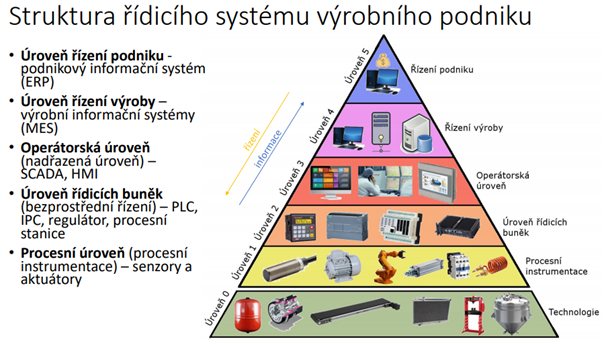
\includegraphics[width=\textwidth]{img/rizeni.png}
    \end{center}
  \end{figure}

\subsubsection*{Úrověň řízení podniku - ERP}
\begin{itemize}
    \item Podnikový informační systém - ERP (= Enterprise Resource Planning).
    \item Zařizuje nákup, logistiku, distribuci, účetnictví, fakturace.
\end{itemize}

\subsubsection*{Úroveň řízení výroby - MES}
\begin{itemize}
    \item Výrobní informační systém - MES (= Matufacturing Execution System).
    \item Shromažďuje data o výrobě a na základě těchto dat posílá příkazy do jednotlivých částí výroby.
    \item Věnuje se například správě výrobních zdrojů, plánováním výroby, řízení výroby, sběr dat, kontrola jakosti, výkonnostní analýzy.
\end{itemize}

\subsubsection*{Operátorská úroveň - SCADA, HMI}
\begin{itemize}
    \item Systém SCADA (= Supervisory Control And Data Acquisition), HMI (= Human Machine Interface) - nadřazená úroveň PLC.
    \item SCADA je vzdálený monitorovací systém - například velín. Jedná se o software monitorující průmyslová a technická zařízení, jejich procesy a umožňuje vzdálené ovládání.
    \item HMI je dotyková obrazovka, umožňující ovládání a monitorování procesu přímo u daného zařízení. 
    \item Lidská činnost - definování procesu, hlídání chybových hlášení, správa atp.
\end{itemize}

\subsubsection*{Úroveň řídícíh buněk}
\begin{itemize}
    \item Bezprostřední řízení procesů pomocí PLC, IPC, regulátory, procesní stanice.
    \item Systémy přímo napojené na výrobní prostředek, spravující jeho sledování a nastavování. 
\end{itemize}

\subsubsection*{Procesní úroveň}
\begin{itemize}
    \item Snímače, akční členy (aktuátory), motory, roboti.
    \item Snímače získávají data z výrobního procesu. Akční členy tyto procesy nějakým způsobem ovlivňují. 
\end{itemize}

\subsubsection*{Technologie}
\begin{itemize}
    \item Elektrické přostředky, tepelné zařízení, dopravníkový pás, převodovky,...
\end{itemize}

\subsection{Možnosti propojení úrovní řízení}
\begin{itemize}
    \item ERP - MES = komunikace pomocí ethernetu.
    \item SCADA - PLC = komunikace pomocí ethernetu - například standard OPC UA.
    \item PLC - HMI = komunikace pomocí sériové komunikace, ethernet. Například Modbus TCP, Ethernet/IP, ProfiNET.
    \item PLC - Snímače = propojeny elektronicky (pomocí digitálních/analogových vstupů/výstupů - proudové smyčky 4-20mA), sběrnicí - IO-Link, AS-Interface, Profibus.
\end{itemize}

\subsection{Centralizované a distribuované řízení výroby}
\subsubsection*{Distribuované - DCS}
\begin{itemize}
    \item DCS = Distributed Control System.
    \item Každá řídící komponenta má na starost svou dílčí oblast, která je do jisté míry autonomní - například PLC.
    \item Tyto komponenty komunikují mezi sebou, případně s nadřazeným systémem, který je ovládá jako celek.
\end{itemize}

\subsubsection*{Centralizované}
\begin{itemize}
    \item Řízení z jednoho organizačního ústředí = jeden řídící komponent, kde se vyhodnocuje logika pro řízení všech procesů.
\end{itemize}

\begin{figure}[h]
    \begin{center}
      \includegraphics[scale = 1]{img/picture2.png}
    \end{center}
  \end{figure}

  \subsection{Toky dat a druhy řízení}
  V principu ERP zapisuje do MES požadavky na výrobu, MES podle požadavku nastavuje výrobní prostředky. Z výrobních prostředků se vrací informace o jejich stavu (výkonnost, opotřebení, spotřeba materiálu), které MES nějakým způsobem zaobaluje, aby tyto informace byly „použitelné pro business“.

  \begin{figure}[h]
    \begin{center}
      \includegraphics[scale = 1]{img/picture3.png}
    \end{center}
  \end{figure}


  \subsection{Vlastnosti a možnosti nadřazených výrobních systémů (MES,ERP)}
  \subsubsection*{ERP}
  \begin{itemize}
    \item Slouží k řízení podniku, obchodní část systémů, logistika, distribuce, správa majetku, faktury, učetnictví,\dots
    \item Výhody:\begin{itemize}
        \item Zefektivnění a zrychlení podnikových procesů
        \item Centralizace a vyčištění dat, snížení chybovosti
        \item Méně byrokracie
        \item Vyšší bezpečnost
    \end{itemize}
    \item Funkce: \begin{itemize}
        \item Vyřizování objednávek
        \item Nákup materiálu
        \item Zajišťování lidských zdrojů
        \item Výpočet ziskovosti
        \item Prodej a distribuce produktů
    \end{itemize}
  \end{itemize}

  \subsection{MES}
  \begin{itemize}
    \item Informační a řídící systém podporující efektivní provádění výrobních operací.
    \item Sbírá aktuální a přesná data, navádí a spouští aktivity v závodě a podává informace "výš".
    \item Funkce: \begin{itemize}
        \item Správa výrobních zdrojů a postupů
        \item Plánování výroby a řízení ze strany dispečera
        \item Jakostní a výkonnostní analýzy
        \item Sběr dat
    \end{itemize}
    \item Spolupráce s ERP: \begin{itemize}
        \item Nastavení výroby dle požadavků ERP - množství, kvalita, receptura = možnosti výroby.
    \end{itemize}
  \end{itemize}
